\documentclass[12pt,a4paper]{article}
\usepackage[utf8]{inputenc}
\usepackage[T1]{fontenc}
\usepackage[french]{babel}
\usepackage{times}
\usepackage{graphicx}
\usepackage{geometry}
\geometry{left=2.5cm, right=2.5cm, top=2.5cm, bottom=2.5cm}
\usepackage{setspace}
\onehalfspacing
\usepackage{hyperref}
\hypersetup{
    colorlinks=true,
    linkcolor=black,
    urlcolor=blue,
}
\usepackage{enumitem}
\usepackage{longtable}
\usepackage{caption}
\usepackage{array}
\usepackage{multirow}
\usepackage{fancyhdr}
\usepackage{lastpage}
\usepackage{float}
\usepackage{chngcntr}
\counterwithin{section}{chapter}
\usepackage{booktabs}
\usepackage{titlesec}
\titleformat{\chapter}
{\normalfont\huge\bfseries}
{\thechapter}{1em}{}

\pagestyle{fancy}
\fancyhf{}
\fancyhead[L]{SAD-ALERTE - Mémoire de Licence}
\fancyfoot[C]{\thepage/\pageref{LastPage}}
\renewcommand{\headrulewidth}{0.4pt}
\renewcommand{\footrulewidth}{0.4pt}

\begin{document}

% Page de garde
\begin{titlepage}
    \begin{center}
        \vspace*{0.5cm}
        \begin{minipage}[t]{0.45\textwidth}
            \begin{flushleft}
                
\includegraphics[width=0.25\textwidth]{media/image1.jpeg}
            \end{flushleft}
        \end{minipage}
        \hfill
        \begin{minipage}[t]{0.45\textwidth}
            \begin{flushleft}
                
\includegraphics[width=0.6\textwidth]{media/image2.jpeg}
                
                \vspace{0.2cm}
                \textbf{\small La patrie ou la mort nous vaincrons}
            \end{flushleft}
        \end{minipage}
        
        \vspace{2cm}
        \textbf{\Huge CONCEPTION ET RÉALISATION D'UN SYSTÈME D'ALERTE DANS LES ZONES À FORT DÉFI SÉCURITAIRE AU BURKINA}
        
        \vspace{2cm}
        \textbf{\Large Mémoire présenté pour l'obtention de la Licence en Informatique}
        
        \vspace{1.5cm}
        \textbf{Présenté par :} \\
        \textbf{\Large OUEDRAOGO Moumouni}
        
        \vspace{1cm}
        \textbf{Sous la direction de :} \\
        \textbf{\Large Dr Philippe KAHOUN} \\
        \large Enseignant-chercheur à BIT
        
        \vspace{0.8cm}
        \textbf{Année académique : 2025-2026}
    \end{center}
\end{titlepage}

% Pages préliminaires en chiffres romains
\pagenumbering{roman}
\setcounter{page}{1}

% Dédicace
\newpage
\phantomsection
\addcontentsline{toc}{section}{DÉDICACE}
\section*{DÉDICACE}
\vspace{1cm}
\begin{center}
    \textit{Je dédie ce travail à mes parents !}
\end{center}

% Remerciements
\newpage
\phantomsection
\addcontentsline{toc}{section}{REMERCIEMENTS}
\section*{REMERCIEMENTS}
\vspace{1cm}
Je tiens à exprimer ma profonde gratitude à toutes les personnes qui ont contribué, de près ou de loin, à la réalisation de ce mémoire.\\
Mes remerciements vont en premier lieu à l'administration de Burkina Institute of Technology (BIT) et à l'ensemble du corps enseignant du département d'Informatique pour la qualité de la formation dispensée.\\
Je remercie tout particulièrement mon Directeur de Mémoire, Dr Philippe KAHOUN, Enseignant chercheur à BIT, pour son encadrement précieux, ses conseils avisés et sa disponibilité.\\
Enfin, j'adresse mes remerciements à mes camarades de classe, ainsi qu'à mes amis et à ma famille pour leur soutien indéfectible.

% Résumé (page séparée)
\newpage
\phantomsection
\addcontentsline{toc}{section}{RÉSUMÉ}
\section*{RÉSUMÉ}
\vspace{1cm}
Ce mémoire propose la conception et la réalisation d'un système d'alerte précoce des menaces sécuritaires au Burkina Faso. Face à la crise sécuritaire depuis 2015 et aux limites des approches réactives, la solution développée intègre un module d'import de rapports administratifs, un système hybride de localisation (GPS/saisie manuelle), un apprentissage automatique basé sur les imports, et une gestion dynamique des seuils par IA. Des mécanismes à plusieurs niveaux détectent les fausses informations. L'implémentation repose sur une architecture backend Node.js/Express, une base de données PostgreSQL/PostGIS, et un frontend React/Next.js. Des maquettes illustrent l'ensemble des fonctionnalités. Les premières évaluations montrent des résultats encourageants.

\paragraph{Mots-clés :} Système d'aide à la décision ; Alerte précoce ; Sécurité ; Apprentissage automatique ; Détection de fausses informations

% Abstract (page séparée)
\newpage
\phantomsection
\addcontentsline{toc}{section}{ABSTRACT}
\section*{ABSTRACT}
\vspace{1cm}
This thesis proposes the design and implementation of an early warning system for security threats in Burkina Faso. Faced with the security crisis since 2015 and the limitations of reactive approaches, the developed solution integrates an administrative report import module, a hybrid localization system (GPS/manual entry), machine learning based on imports, and dynamic threshold management by AI. Multi‑level mechanisms detect false information. The implementation is based on a Node.js/Express backend, a PostgreSQL/PostGIS database, and a React/Next.js frontend. Mockups illustrate all functionalities. Initial evaluations show encouraging results.

\paragraph{Keywords:} Decision support system ; Early warning ; Security ; Machine learning ; Fake news detection

% Table des matières (sans auto‑référence)
\newpage
\renewcommand{\contentsname}{}
\tableofcontents

% Liste des acronymes
\newpage
\phantomsection
\addcontentsline{toc}{section}{LISTE DES ACRONYMES}
\section*{LISTE DES ACRONYMES}
\vspace{1cm}
\begin{longtable}{p{3cm}p{10cm}}
\textbf{2FA} & Two-Factor Authentication (Double authentification) \\
\textbf{API} & Application Programming Interface \\
\textbf{CEDEAO} & Communauté Économique des États de l'Afrique de l'Ouest \\
\textbf{DBSCAN} & Density-Based Spatial Clustering of Applications with Noise \\
\textbf{ETL} & Extract, Transform, Load \\
\textbf{FAN} & Forces Armées Nationales \\
\textbf{GPS} & Global Positioning System \\
\textbf{IA} & Intelligence Artificielle \\
\textbf{IED} & Engin Explosif Improvisé \\
\textbf{JSON} & JavaScript Object Notation \\
\textbf{JWT} & JSON Web Token \\
\textbf{KPI} & Key Performance Indicator \\
\textbf{NLP} & Natural Language Processing \\
\textbf{OCR} & Optical Character Recognition \\
\textbf{ONG} & Organisation Non Gouvernementale \\
\textbf{PostGIS} & Extension spatiale de PostgreSQL \\
\textbf{REST} & Representational State Transfer \\
\textbf{SAD} & Système d'Aide à la Décision \\
\textbf{SAP} & Système d'Alerte Précoce \\
\textbf{SIG} & Système d'Information Géographique \\
\textbf{SQL} & Structured Query Language \\
\textbf{UML} & Unified Modeling Language \\
\textbf{VPS} & Virtual Private Server \\
\end{longtable}

% Liste des tableaux
\newpage
\phantomsection
\addcontentsline{toc}{section}{LISTE DES TABLEAUX}
\listoftables

% Liste des figures
\newpage
\phantomsection
\addcontentsline{toc}{section}{LISTE DES FIGURES}
\listoffigures

% Corps du texte en chiffres arabes
\newpage
\pagenumbering{arabic}
\setcounter{chapter}{0}
\setcounter{page}{1}

% INTRODUCTION GÉNÉRALE
\chapter*{INTRODUCTION GÉNÉRALE}
\addcontentsline{toc}{chapter}{INTRODUCTION GÉNÉRALE}

\section*{Contexte de l'étude}
Depuis 2015, le Burkina Faso fait face à une dégradation sécuritaire sans précédent, avec des attaques récurrentes dans les régions du Sahel, de l'Est et du Nord. Cette crise multidimensionnelle a causé des milliers de morts et le déplacement de plus de deux millions de personnes \cite{zongo2020}. Les dispositifs actuels de gestion sécuritaire reposent essentiellement sur des mécanismes réactifs, intervenant après la survenue des incidents.

Parallèlement, l'évolution des technologies numériques (SIG, intelligence artificielle, analyse de données) offre aujourd'hui la possibilité de concevoir des outils d'aide à la décision capables d'anticiper certaines situations à risque. Un gisement d'information précieux est actuellement sous-exploité : les rapports de patrouilles, comptes rendus d'opérations et autres documents administratifs produits quotidiennement par les forces de sécurité.

\section*{Problématique}
Au regard du contexte sécuritaire, la question centrale qui se pose est la suivante : \textbf{comment alerter en cas de menace dans les zones d'insécurité ?}

\section*{Objectifs}
\textbf{Objectif général :} Concevoir un système d'alerte précoce des menaces sécuritaires.

\textbf{Objectifs spécifiques :}
\begin{itemize}
    \item \textbf{Développer une application mobile hybride (en Flutter)} permettant la collecte et le signalement rapide d'incidents sur le terrain, même en zone de faible connectivité.
    \item \textbf{Mettre en place un Backend robuste et une base de données (PostgreSQL)} garantissant le traitement, la sécurité et l'archivage fiable des rapports.
    \item \textbf{Concevoir une interface Web d'administration (en Next.js)} offrant aux décideurs une visualisation dynamique des menaces via une cartographie interactive et des tableaux de bord.
    \item \textbf{Intégrer un moteur d'Intelligence Artificielle (en Python)} chargé de l'analyse prédictive, du filtrage des fausses alertes, et de l'adaptation dynamique des seuils critiques (méthode des 3 sigmas).
\end{itemize}

\section*{Hypothèses de recherche}
\begin{itemize}
    \item \textbf{H1 :} L'exploitation des données historiques améliore la qualité des prédictions.
    \item \textbf{H2 :} Un système hybride de localisation couvre efficacement l'ensemble du territoire.
    \item \textbf{H3 :} La détection multi‑niveaux permet d'identifier un grand nombre de tentatives d'introduction de fausses informations.
    \item \textbf{H4 :} Une gestion dynamique des seuils réduit les fausses alertes tout en maintenant un bon niveau de détection.
\end{itemize}

\section*{Structure du mémoire}
Ce mémoire est structuré en deux parties. La première partie présente les études théoriques (chapitres 1 et 2). La seconde partie détaille la conception, l'implémentation et l'évaluation (chapitres 3 et 4).

% PARTIE I
\newpage
\vspace*{\fill}
\begin{center}
    \Huge \textbf{PARTIE I : ÉTUDES THÉORIQUES}
\end{center}
\vspace*{\fill}
\newpage

\chapter{Chapitre I : Informations générales sur les systèmes d'alerte}

\section{Contexte sécuritaire au Burkina Faso}
Le Burkina Faso connaît depuis 2015 une crise sécuritaire majeure. Les régions du Sahel, de l'Est et du Nord sont les plus touchées. Les facteurs explicatifs incluent la fragilité des frontières, la présence de groupes armés issus du conflit malien, les tensions communautaires, et la faiblesse des systèmes d'information et d'anticipation.

\section{Concepts fondamentaux de l'alerte précoce}
Un système d'alerte précoce (SAP) repose sur quatre piliers \cite{nationsunies2006} : la connaissance du risque, le suivi et la détection, la communication et la diffusion, et la capacité de réponse. Dans le contexte sécuritaire, il vise à détecter les signaux faibles (regroupements suspects, mouvements inhabituels) avant qu'ils ne se transforment en attaque.

\section{SIG et systèmes d'aide à la décision}
Les systèmes d'information géographique (SIG) permettent de visualiser et d'analyser des données géographiques \cite{longley2015}. Leurs fonctionnalités clés sont la visualisation (cartes dynamiques), l'analyse spatiale (corrélations, tendances), et la gestion des ressources.

Les systèmes d'aide à la décision (SAD) sont des systèmes interactifs qui aident les décideurs à utiliser des données et des modèles pour résoudre des problèmes complexes \cite{turban2015}.

\section{Apprentissage automatique pour la prédiction sécuritaire}
L'apprentissage automatique permet d'identifier des patterns dans les données historiques, de prédire les zones à risque, et de détecter des anomalies \cite{geron2022}. Les techniques adaptées incluent les forêts aléatoires pour la classification, DBSCAN pour la détection de clusters, et Isolation Forest pour la détection d'anomalies.

\section{Solutions existantes}
Au niveau international, des systèmes comme PredPol utilisent l'analyse prédictive. Au niveau africain, la CEDEAO dispose d'un système d'alerte précoce. Aucune solution n'est directement transposable au Burkina Faso sans adaptation aux réalités locales.


\newpage
\chapter{Chapitre II : Méthodologies et approches conceptuelles}

\section{Mécanismes réactifs en place}
Actuellement, le système de gestion des incidents sécuritaires repose de manière prédominante sur des mécanismes réactifs. Les Forces de Défense et de Sécurité (FDS) s'appuient principalement sur des rapports hiérarchiques manuscrits ou numérisés a posteriori, ainsi que sur les retours réguliers des patrouilles de terrain. Par ailleurs, les comités de vigilance locaux et les Volontaires pour la Défense de la Patrie (VDP) jouent un rôle crucial de renseignement à la base. Cependant, les informations qu'ils remontent souffrent souvent d'un manque de structuration et de standardisation. En parallèle, les Organisations Non Gouvernementales (ONG) et les médias locaux apportent des données complémentaires, bien que celles-ci restent très hétérogènes et difficiles à agréger en temps réel.

\section{Limites identifiées}
\begin{table}[H]
\centering
\caption{Synthèse des limites des systèmes actuels}
\begin{tabular}{|l|l|l|}
\hline
\textbf{Catégorie} & \textbf{Limites} & \textbf{Impact} \\
\hline
Données & Fragmentées, hétérogènes & Pas de vision globale \\
\hline
Analyse & Manuelle, rétrospective & Pas d'anticipation \\
\hline
Localisation & Dépendance au GPS & Angles morts \\
\hline
Seuils & Statiques & Inadaptés au contexte \\
\hline
Historique & Archives non exploitées & Modèles non optimisés \\
\hline
\end{tabular}
\end{table}

\section{Risques liés aux fausses informations}
Dans un contexte de guerre asymétrique, la gestion de l'information est devenue un enjeu stratégique majeur. Les systèmes d'alerte font face à de nombreux risques liés à l'injection de données erronées. Parmi ces menaces, nous retrouvons la diversion, qui consiste à déclencher de fausses alertes pour éloigner les forces de sécurité de leur cible réelle. La dissimulation et l'amplification permettent quant à elles de manipuler la perception du danger. Par ailleurs, des adversaires peuvent recourir à l'usurpation d'identité ou à la saturation du système par un afflux massif de signalements inutiles. Les conséquences de ces manipulations peuvent être désastreuses, allant du gaspillage critique des ressources logistiques à la perte de crédibilité du système, et dans le pire des cas, à la perte de vies humaines.

\section{Synthèse des besoins}
Afin de pallier les insuffisances des mécanismes actuels, nous avons dégagé plusieurs besoins majeurs pour la conception de notre système. 

\textbf{Besoins fonctionnels :} Le système doit impérativement permettre la centralisation sécurisée des données en un point unique. Il doit intégrer un module d'import de documents administratifs pour numériser les archives existantes. De plus, il est crucial de mettre à disposition une localisation hybride (GPS et saisie manuelle) pour s'adapter aux zones sans couverture réseau. Enfin, l'application doit embarquer des algorithmes d'apprentissage automatique pour le calcul de seuils adaptatifs, tout en assurant une détection proactive des tentatives de manipulation de l'information.

\textbf{Besoins non fonctionnels :} Sur le plan technique, l'application doit garantir un haut niveau de sécurité pour protéger l'identité des signalants. Elle doit faire preuve de résilience face aux pannes de réseau, offrir une grande adaptativité selon l'évolution du contexte, et maintenir une accessibilité maximale pour les agents disposant de terminaux mobiles aux performances limitées.

% PARTIE II
\newpage
\vspace*{\fill}
\begin{center}
    \Huge \textbf{PARTIE II : CONCEPTION ET RÉALISATION}
\end{center}
\vspace*{\fill}
\newpage


\chapter{Chapitre I : Conception, modélisation et approche conceptuelle}

\section{Architecture générale du système}
L'architecture du système repose sur trois couches distinctes :

\textbf{Couche présentation} : développée avec React/Next.js, elle offre des interfaces adaptées à chaque profil d'utilisateur (agent terrain, analyste, décideur, administrateur). L'application est responsive et fonctionne sur ordinateur, tablette et smartphone.

\textbf{Couche services} : implémentée avec Node.js/Express, elle regroupe les fonctionnalités métier : import de documents, géocodage, apprentissage automatique, gestion des seuils, détection des manipulations. Les API REST assurent la communication avec le frontend.

\textbf{Couche données} : basée sur PostgreSQL avec l'extension PostGIS pour les données spatiales, elle inclut un entrepôt historique, un cache Redis pour les performances, et un référentiel géographique des localités burkinabè.

\section{Modélisation UML}
\subsection{Diagramme de cas d'utilisation}
Ce diagramme présente les interactions principales entre les différents acteurs du système (Agent de terrain, Analyste, Décideur et Administrateur) et les fonctionnalités offertes par la plateforme. Il met en évidence les actions clés telles que l'authentification sécurisée, la soumission de signalements, la validation des extractions, et l'accès au tableau de bord pour la prise de décision.
\begin{figure}[H]
    \centering
    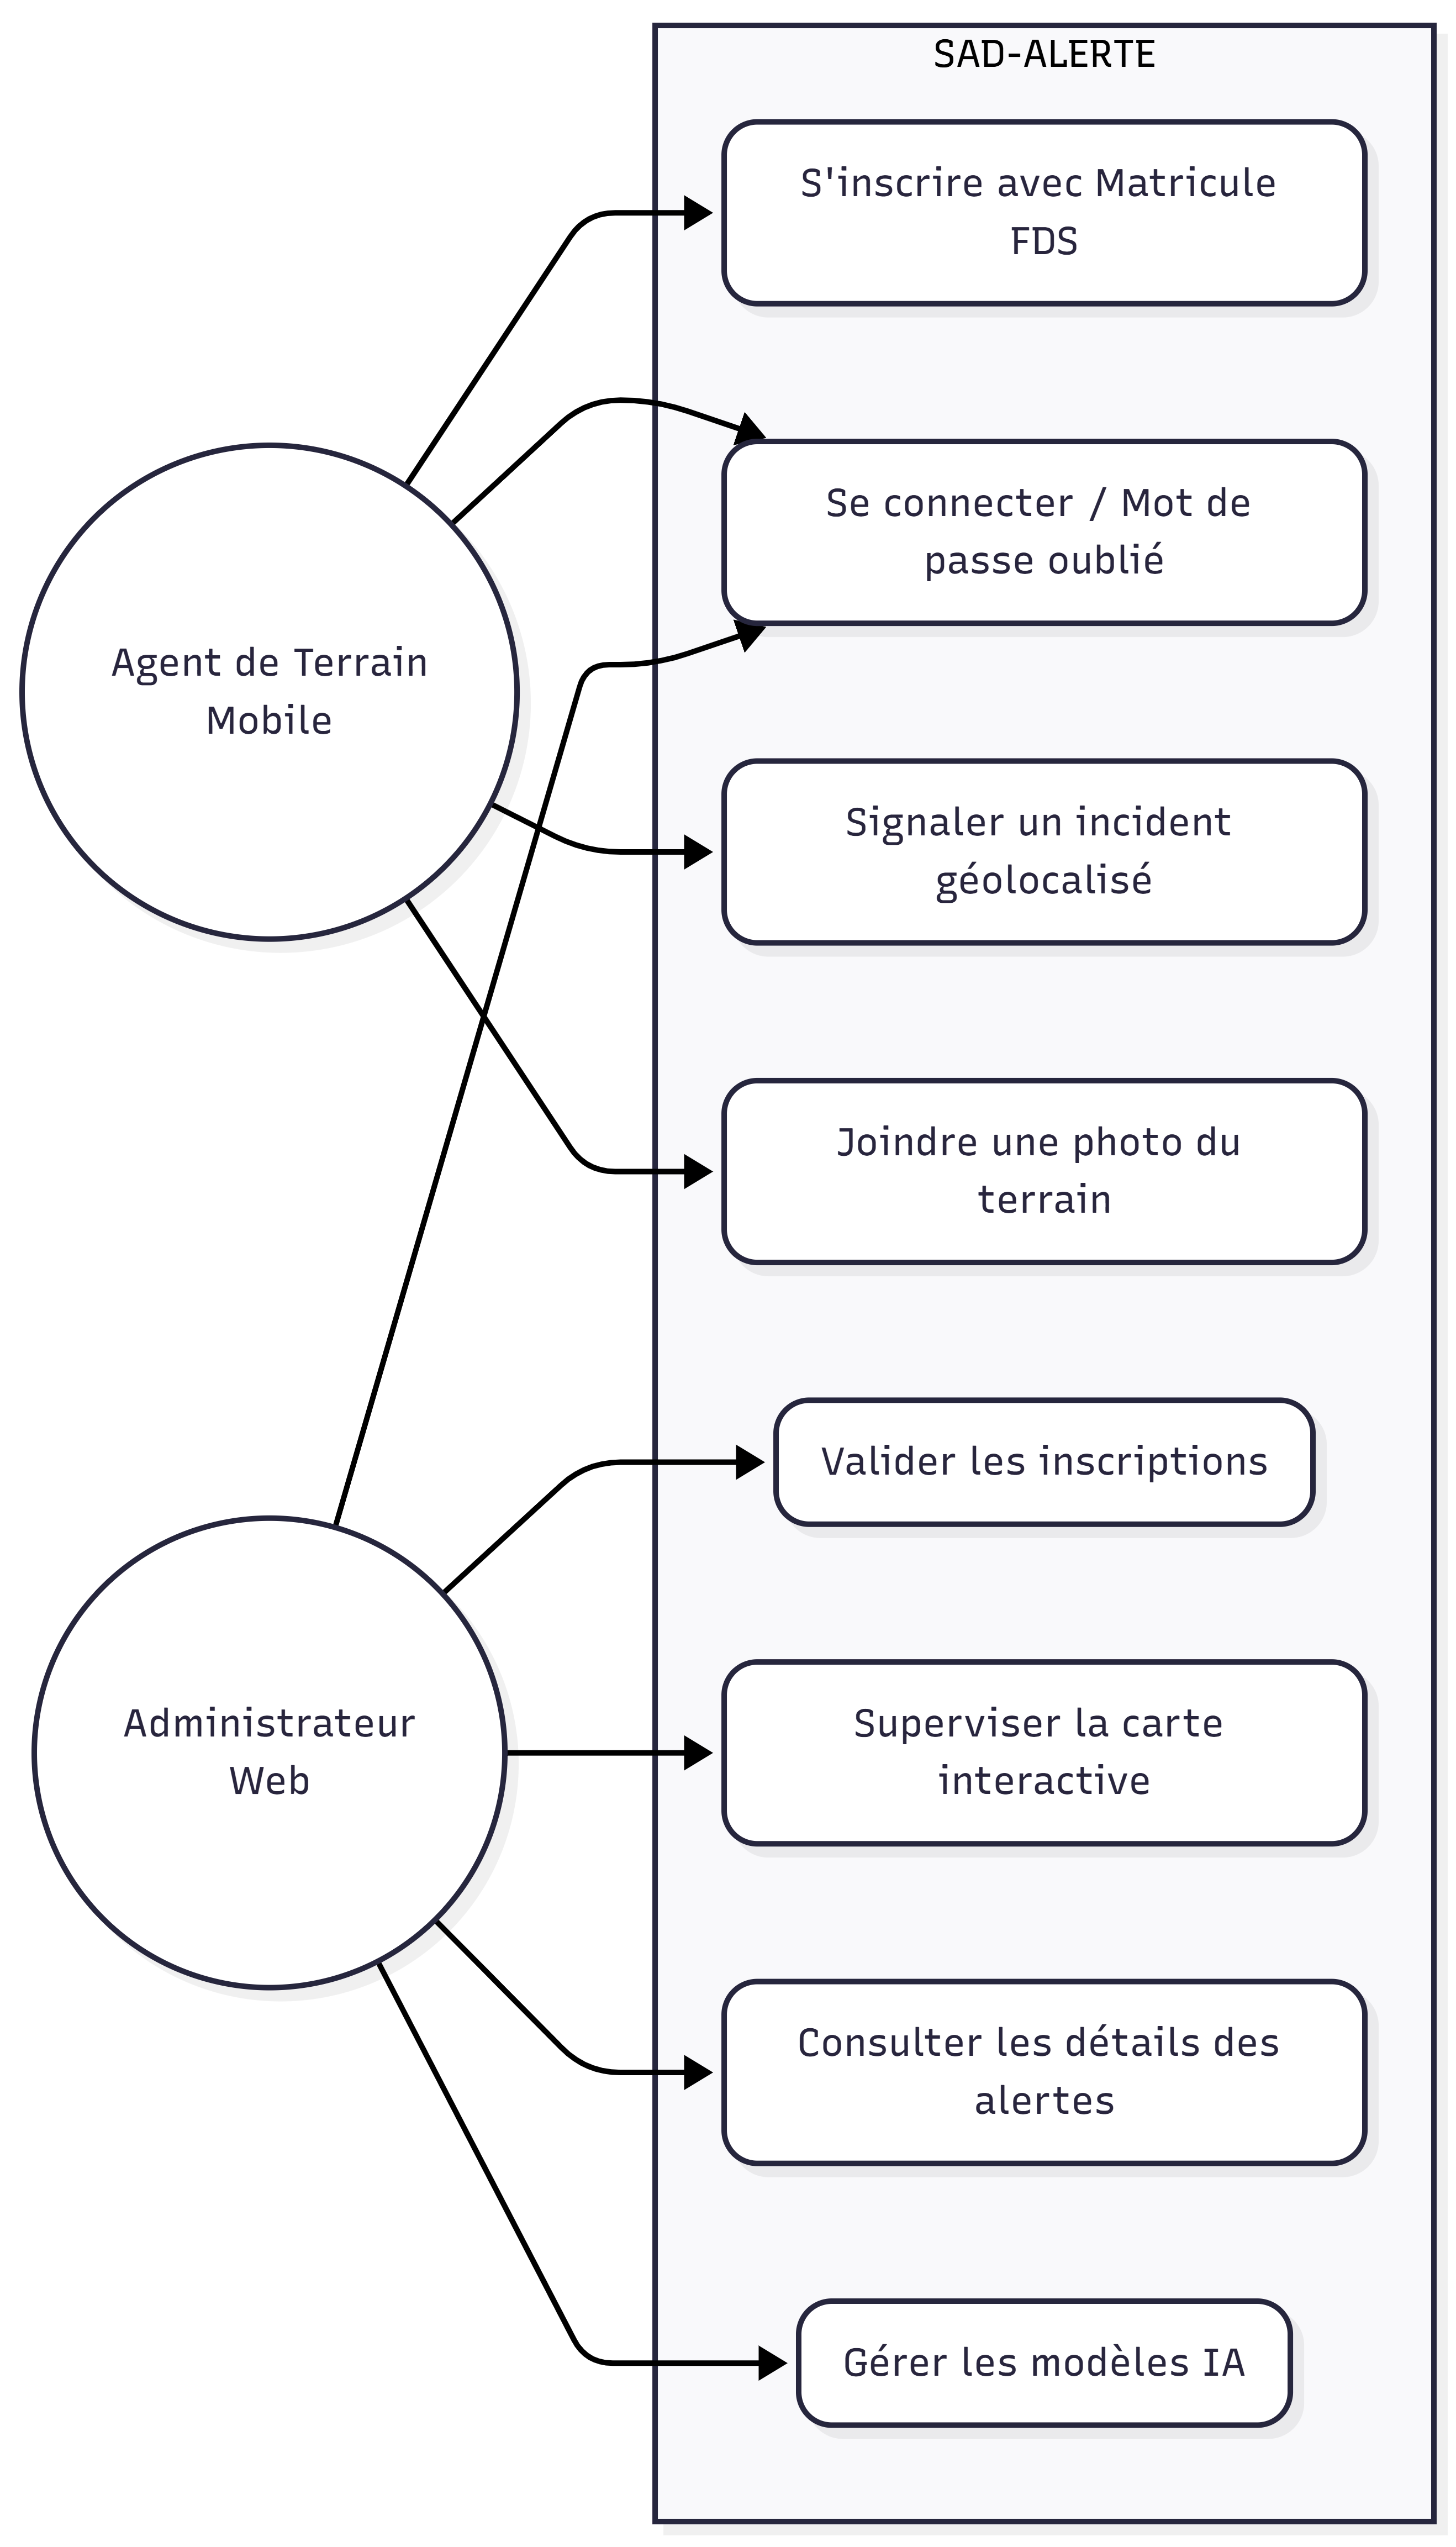
\includegraphics[width=0.8\textwidth]{media/use_case.png}
    \caption{Diagramme de cas d'utilisation}
\end{figure}

\subsection{Diagramme de classes UML}
Le diagramme de classes (qui sert également de Modèle Conceptuel de Données) détaille l'architecture des données du système. Il identifie les entités fondamentales telles que \textit{Utilisateur}, \textit{Incident}, \textit{Alerte}, \textit{Rapport} et \textit{Localité}, en précisant leurs attributs respectifs ainsi que les relations de cardinalité qui les lient.
\begin{figure}[H]
    \centering
    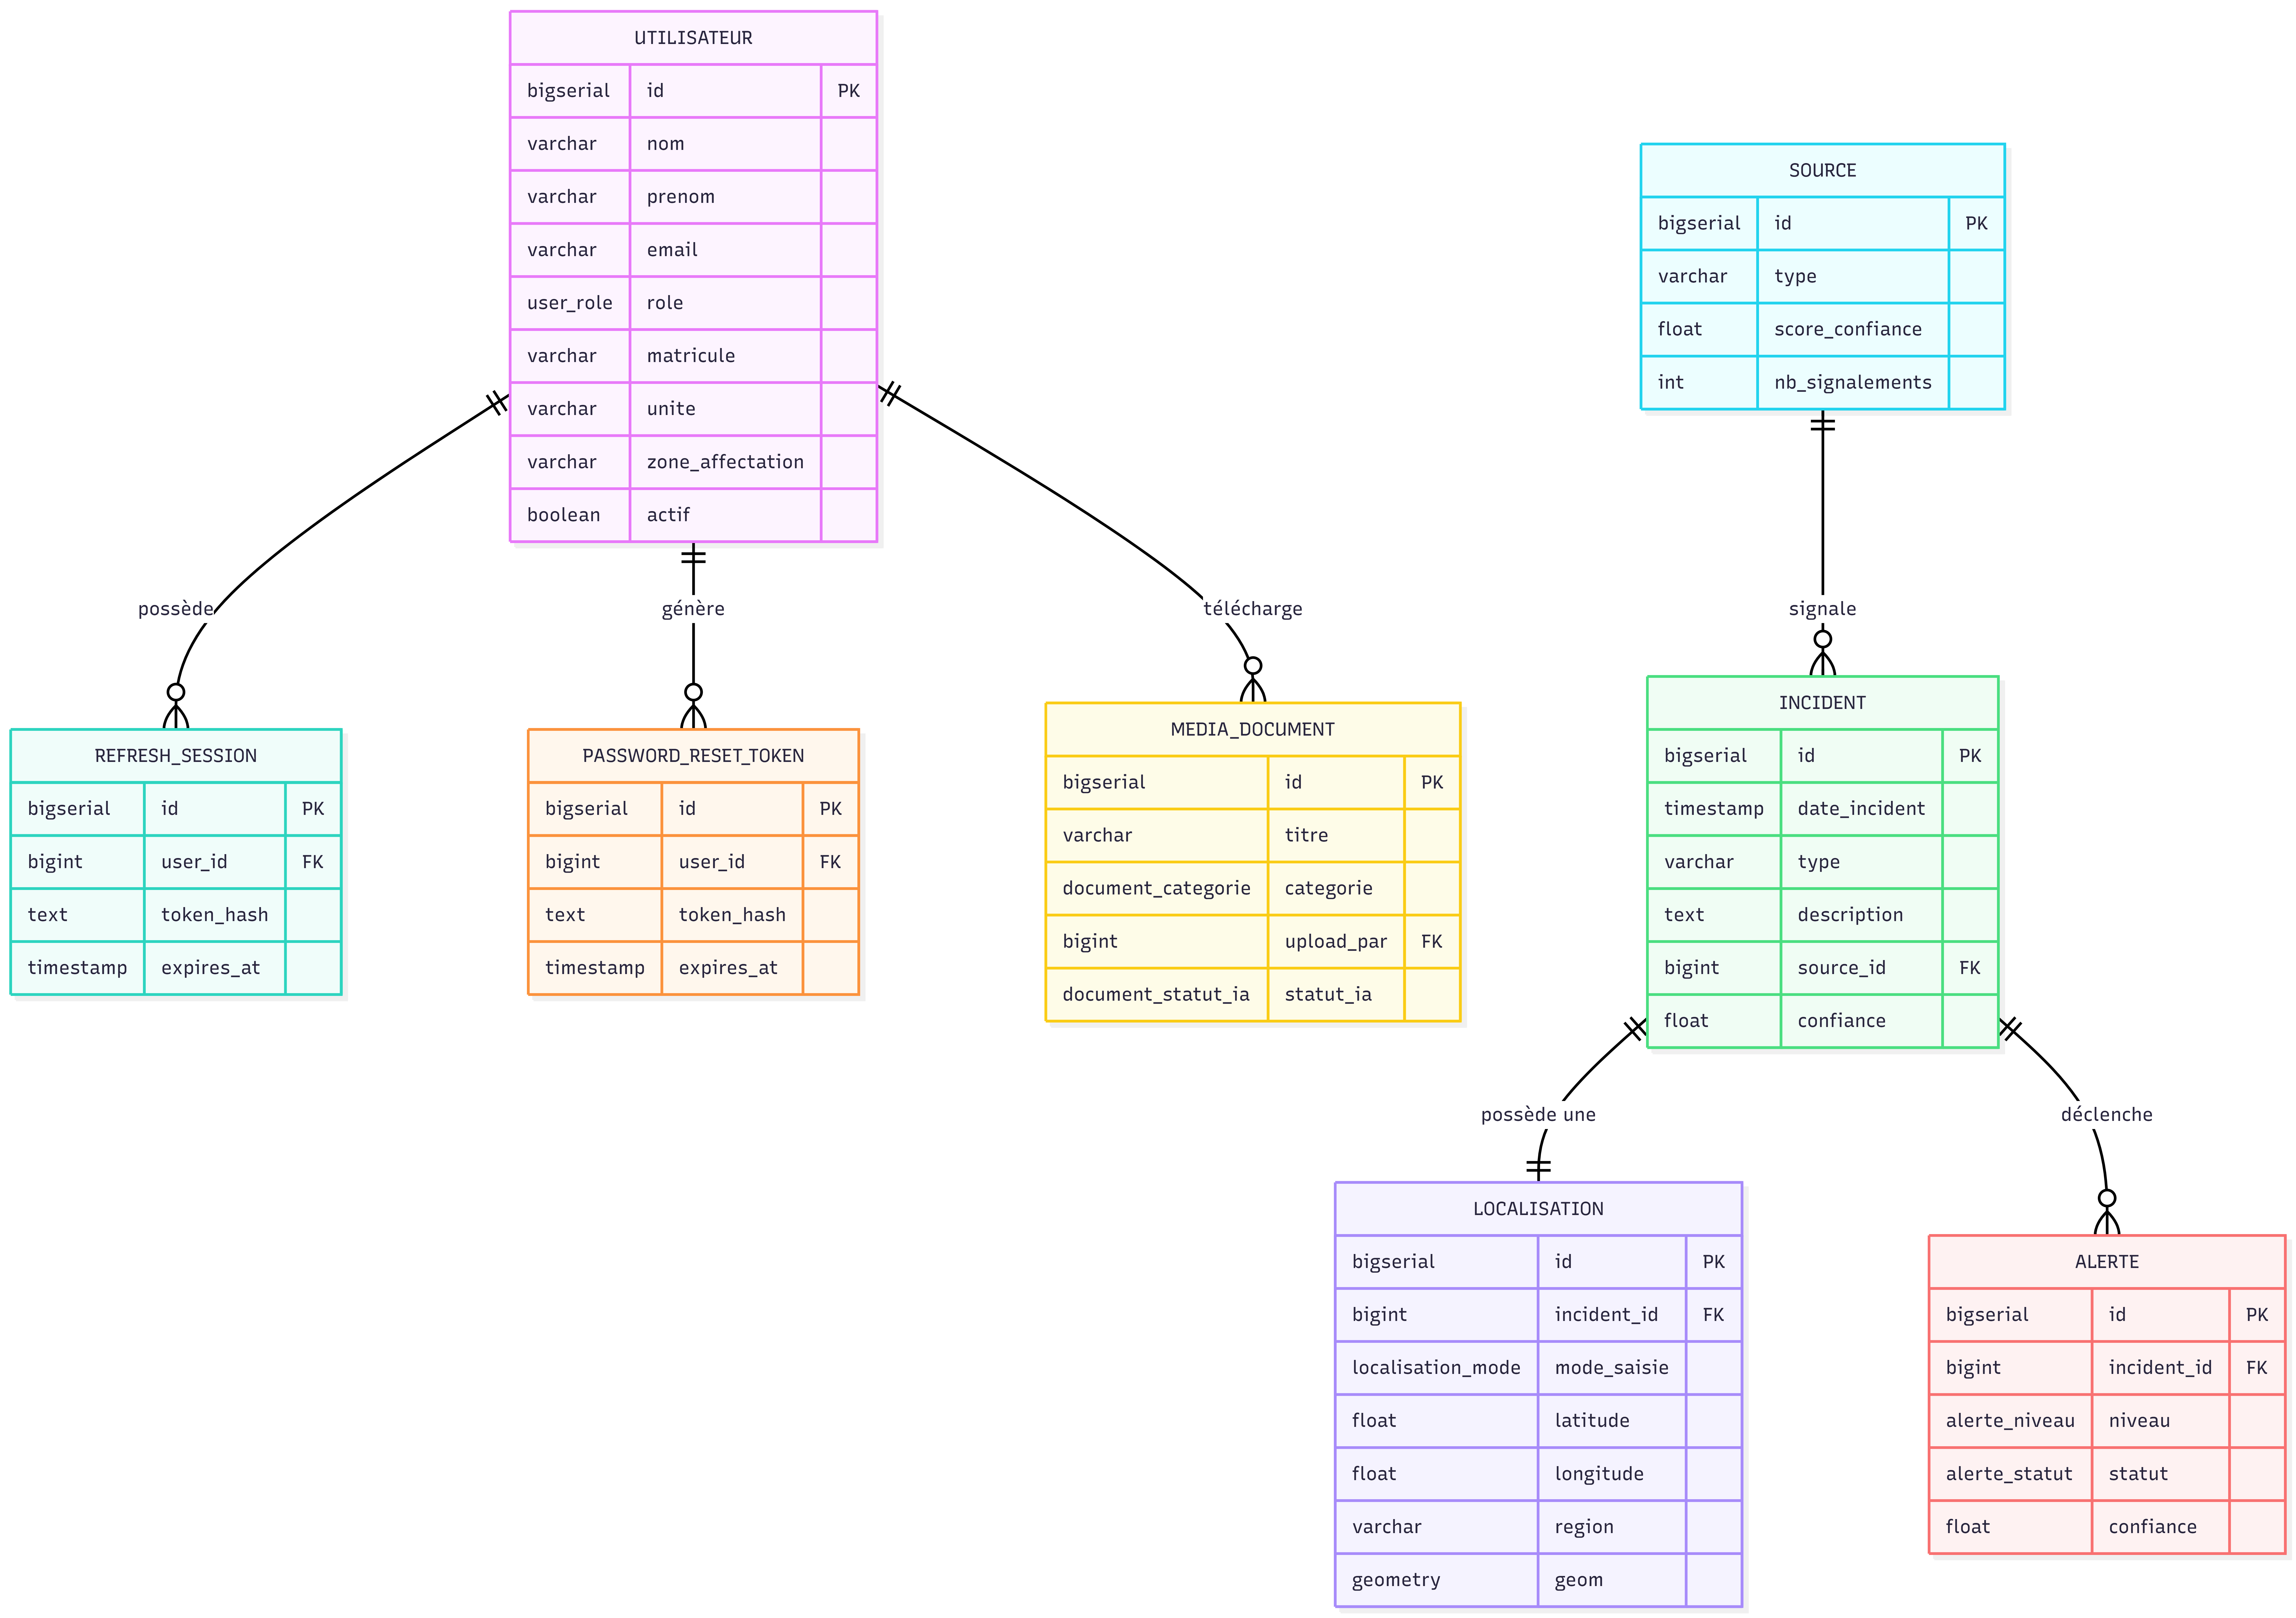
\includegraphics[width=1\textwidth]{media/class_diagram.png}
    \caption{Modèle Conceptuel de Données (MCD) / Diagramme de classes}
\end{figure}

\subsection{Diagramme de séquence}
Ce diagramme illustre la dynamique temporelle et la chronologie des échanges de messages entre les différents composants (Application Mobile, Serveur Backend, Moteur IA, et Base de données). Il retrace spécifiquement le flux d'exécution lors du signalement d'un incident, incluant la vérification, le calcul des seuils par l'IA et le déclenchement potentiel d'une alerte critique.
\begin{figure}[H]
    \centering
    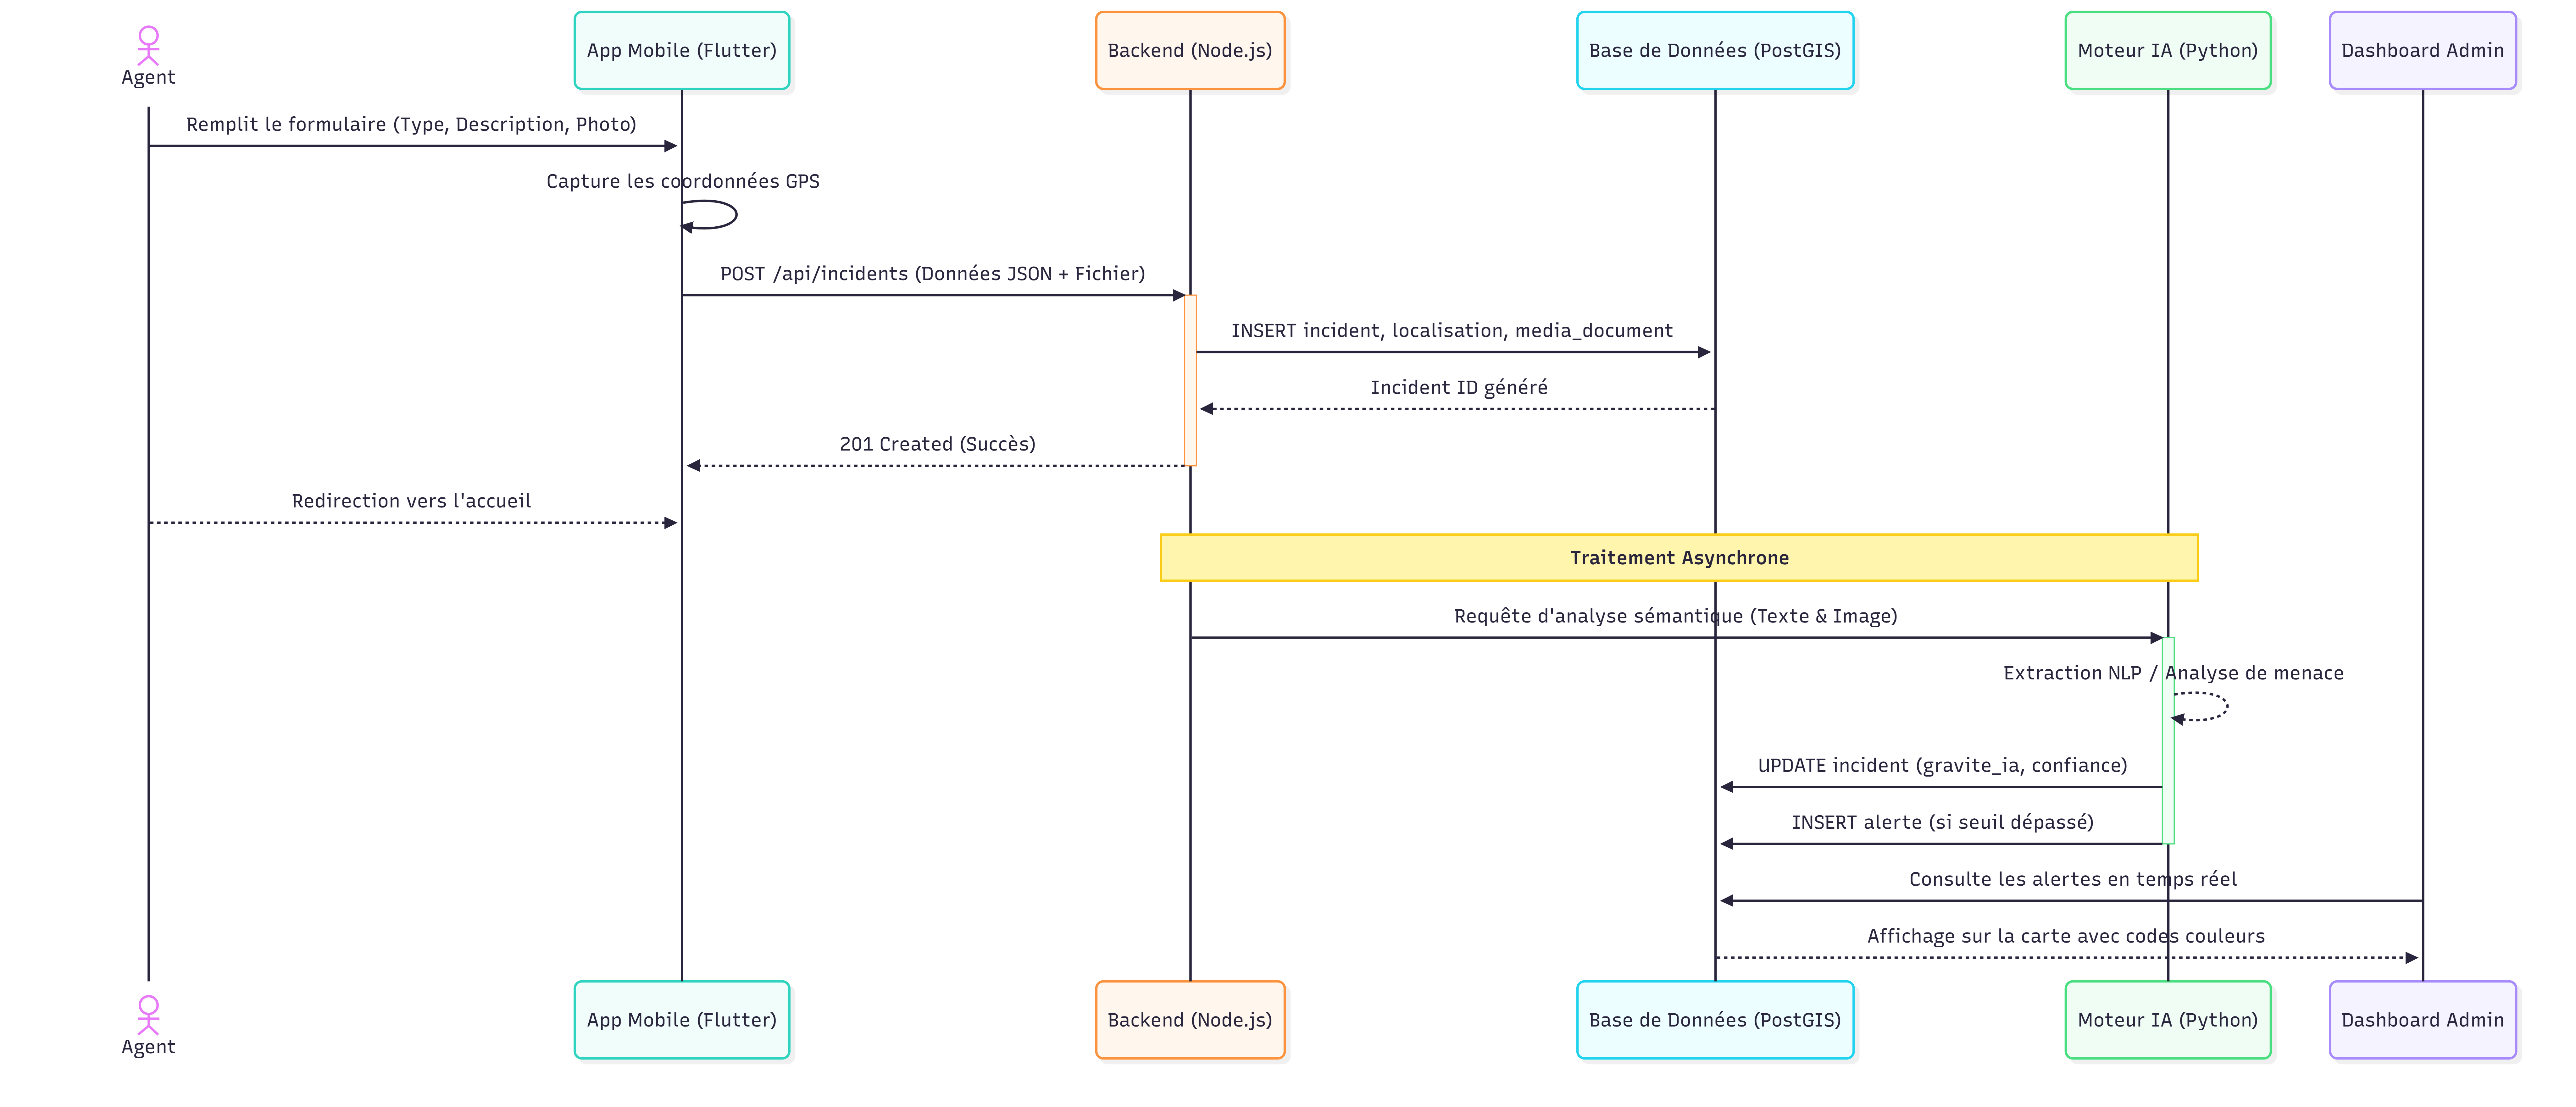
\includegraphics[width=1\textwidth]{media/sequence.png}
    \caption{Diagramme de séquence global du système}
\end{figure}

\section{Structure de la base de données (Schéma SQL)}
La figure ci-dessous représente le schéma d'implémentation physique de la base de données sous PostgreSQL couplée à PostGIS. Elle expose la définition des tables, les contraintes d'intégrité (clés primaires et étrangères), ainsi que les types de données spatiaux (géométrie) essentiels pour le requêtage et le traitement géospatial des incidents rapportés.
\begin{figure}[H]
    \centering
    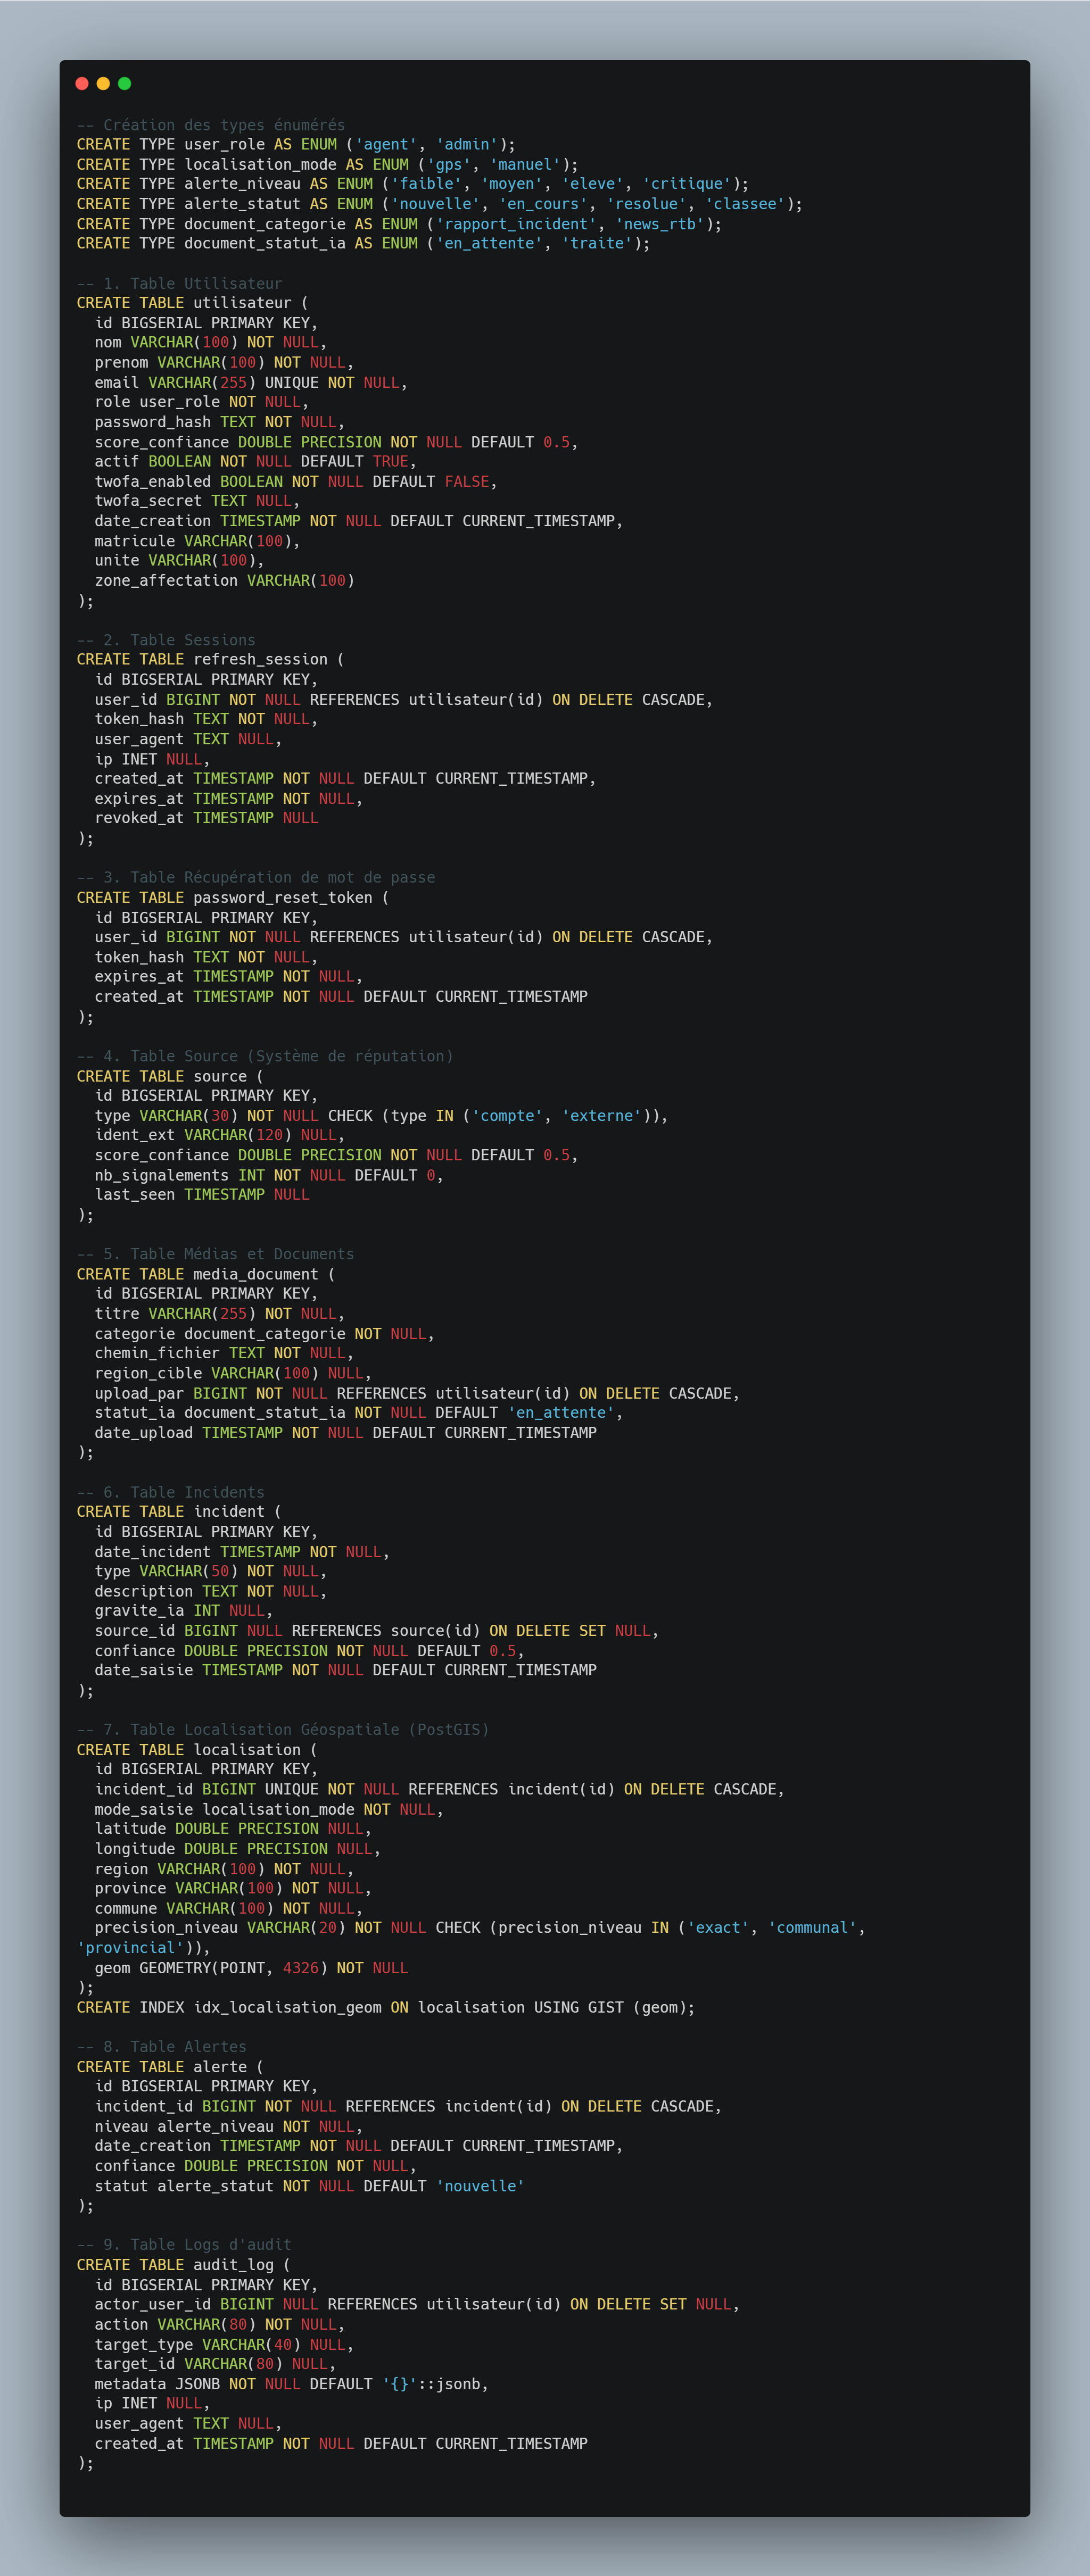
\includegraphics[width=\textwidth,height=0.45\textheight,keepaspectratio]{media/db_schema.png}
    \caption{Schéma relationnel et code SQL de création des tables}
\end{figure}

\section{Système hybride de localisation}
\begin{table}[H]
\centering
\caption{Niveaux de précision de la localisation}
\begin{tabular}{|l|l|l|}
\hline
\textbf{Niveau} & \textbf{Mode} & \textbf{Utilisation} \\
\hline
Exact & GPS & Zones avec réseau, smartphones \\
\hline
Communal & Manuel & Zones sans réseau, téléphones basiques \\
\hline
Provincial & Manuel & Information vague \\
\hline
\end{tabular}
\end{table}

Pour les signalements sans GPS, le système calcule automatiquement un centroïde.

\section{Mécanismes de détection des fausses informations}
Afin d'assurer la fiabilité des données collectées, le système implémente une procédure stricte de vérification reposant sur trois niveaux distincts. Le premier niveau est un filtrage technique qui s'assure de l'intégrité de la requête et de la validité des coordonnées géographiques. Le deuxième niveau consiste en une analyse comportementale du signalant, qui attribue un score de confiance basé sur l'historique de l'utilisateur. Enfin, le troisième niveau est une analyse croisée de convergence, qui recoupe de multiples signalements similaires émanant de sources indépendantes pour confirmer un événement avant de déclencher une alerte formelle.

\section{Gestion dynamique des seuils par IA}
Dans les systèmes d'alerte classiques, les seuils de déclenchement sont statiques et deviennent rapidement inadaptés. Notre solution intègre une gestion dynamique des seuils pilotée par l'Intelligence Artificielle. Ce mécanisme s'appuie sur la règle statistique des 3 sigmas. L'algorithme analyse en continu la fréquence moyenne des incidents dans une région donnée. Si le nombre de signalements dépasse la moyenne plus trois fois l'écart-type, le système identifie formellement une anomalie statistique et lève une alerte critique, s'adaptant ainsi à la "normalité" spécifique de chaque localité.

\chapter{Chapitre II : Implémentation et résultats}

\section{Implémentation technique détaillée}

La concrétisation de l'architecture proposée a nécessité l'utilisation d'un ensemble de technologies robustes et modernes.

\subsection{Backend avec Node.js et Express}
Le Backend constitue le cœur logique de notre système. Développé en JavaScript avec l'environnement d'exécution Node.js et le framework Express, il permet de gérer de manière asynchrone un grand volume de requêtes simultanées. Ce module expose une API RESTful sécurisée. Il est en charge de l'authentification des utilisateurs, de la vérification des droits d'accès via des JSON Web Tokens (JWT), et du traitement métier avant l'insertion des données en base.

\subsection{Frontend Web avec React et Next.js}
L'interface d'administration a été bâtie à l'aide de React.js et du framework Next.js. Ce choix technologique garantit un rendu côté serveur (SSR) qui accélère le temps de chargement des pages. Le tableau de bord offre une expérience utilisateur fluide, permettant aux décideurs d'interagir en temps réel avec la cartographie des incidents générée via la librairie Leaflet.

\subsection{Application Mobile avec Flutter}
Pour les agents de terrain, nous avons développé une application mobile utilisant le framework Flutter. Ce choix permet de disposer d'une base de code unique compatible avec les systèmes Android et iOS. L'application mobile met l'accent sur la simplicité d'utilisation et intègre des fonctionnalités de mise en cache locale pour supporter la saisie de signalements même lorsque la connexion internet est indisponible.

\subsection{Base de données PostgreSQL et PostGIS}
L'ensemble des données est persisté au sein d'une base de données relationnelle PostgreSQL. Afin de traiter efficacement les problématiques de localisation, nous avons couplé ce SGBD avec son extension spatiale PostGIS. Cette combinaison permet de réaliser des requêtes géographiques complexes, telles que le regroupement d'incidents par rayon ou l'identification d'anomalies de positionnement.

\subsection{Intelligence Artificielle avec Python et Scikit-Learn}
L'analyse des menaces et l'évaluation des seuils sont déléguées à un micro-service écrit en Python. Ce module exploite les librairies spécialisées telles que Scikit-Learn et Pandas. Il se connecte régulièrement à la base de données pour réentraîner les modèles d'apprentissage automatique en fonction des nouvelles données importées, garantissant ainsi un système qui s'améliore de manière autonome avec le temps.

\section{Interface utilisateur et maquettes}

\textbf{Remarque sur l'origine des données :} L'ensemble des données, chiffres et pourcentages présentés dans les figures de cette section proviennent de \textbf{données simulées (jeux de données de test)} que nous avons générées lors du développement. Ces données fictives nous ont permis de tester la configuration du système, d'évaluer les algorithmes d'IA (calcul des seuils dynamiques) et de valider les interfaces avant un potentiel déploiement réel sur le terrain.

Les maquettes illustrent les fonctionnalités clés du système.

\subsection{Interface Mobile (Agent terrain)}
L'application mobile est l'outil principal de collecte de données sur le terrain. L'écran d'authentification (à gauche) assure un accès sécurisé réservé aux agents enregistrés, demandant leur identifiant et mot de passe. L'écran de signalement (à droite) présente un formulaire intuitif permettant à l'agent de documenter un incident : sélection du type d'événement, description, niveau de gravité et géolocalisation. Le système capture les coordonnées GPS automatiquement, mais offre également la possibilité de renseigner manuellement la localité en cas de perte de signal.
\begin{figure}[H]
   \centering
   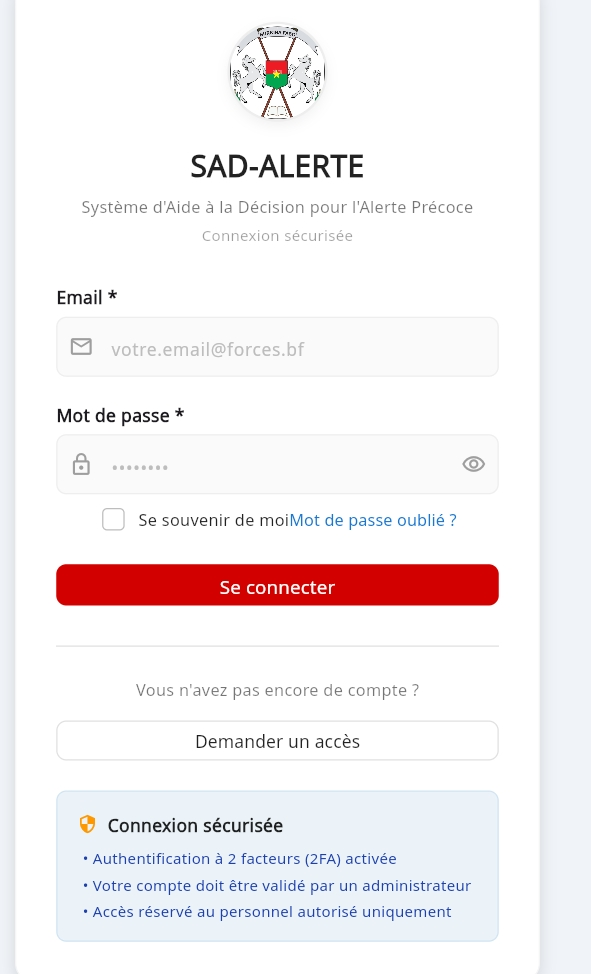
\includegraphics[width=0.4\textwidth]{media/mobile_login.png}
   \hfill
   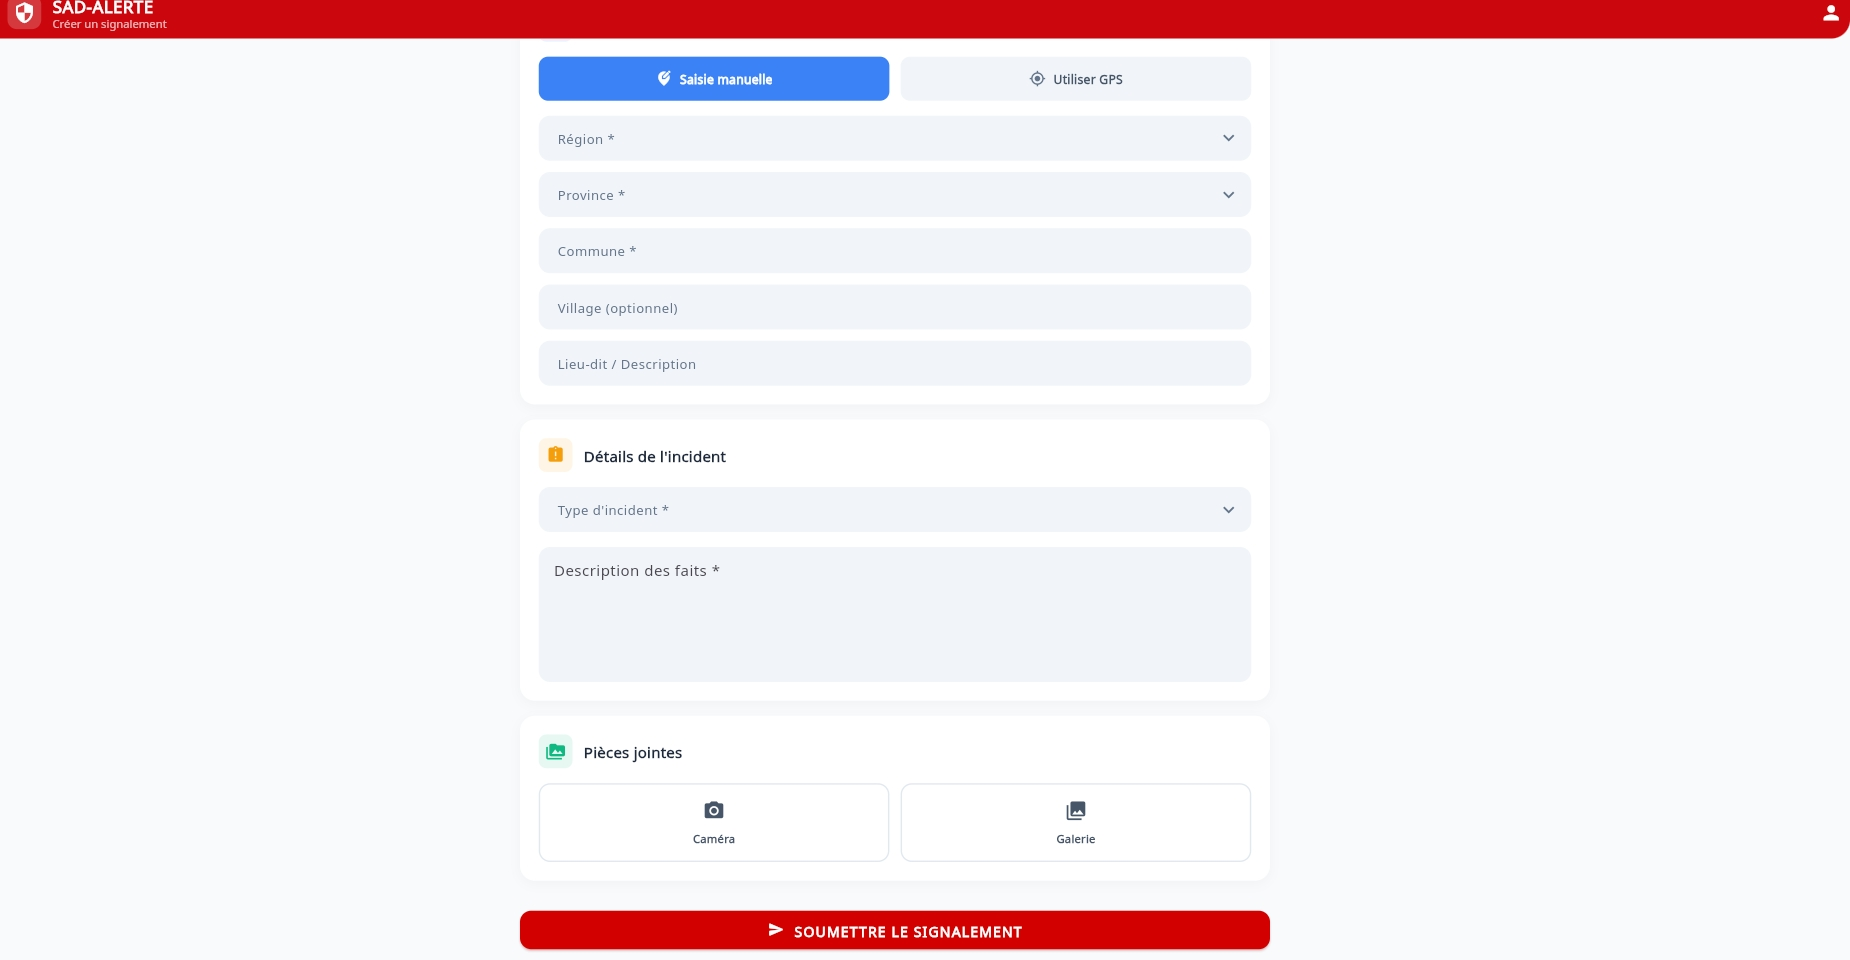
\includegraphics[width=0.4\textwidth]{media/mobile_signalement.png}
   \caption{Application Mobile : Écran de connexion sécurisée et formulaire de signalement hybride}
\end{figure}

\subsection{Tableau de bord et Cartographie}
Le tableau de bord web constitue le centre opérationnel pour les décideurs et les administrateurs. Cette interface présente en haut de page les indicateurs de performance clés (KPIs) tels que le nombre d'incidents signalés, le nombre d'alertes critiques actives et l'état global du système. Au centre, une cartographie interactive dynamique affiche la répartition spatiale des menaces. Les marqueurs et les zones de chaleur (clusters) permettent d'identifier instantanément les foyers d'insécurité sur le territoire national.
\begin{figure}[H]
   \centering
   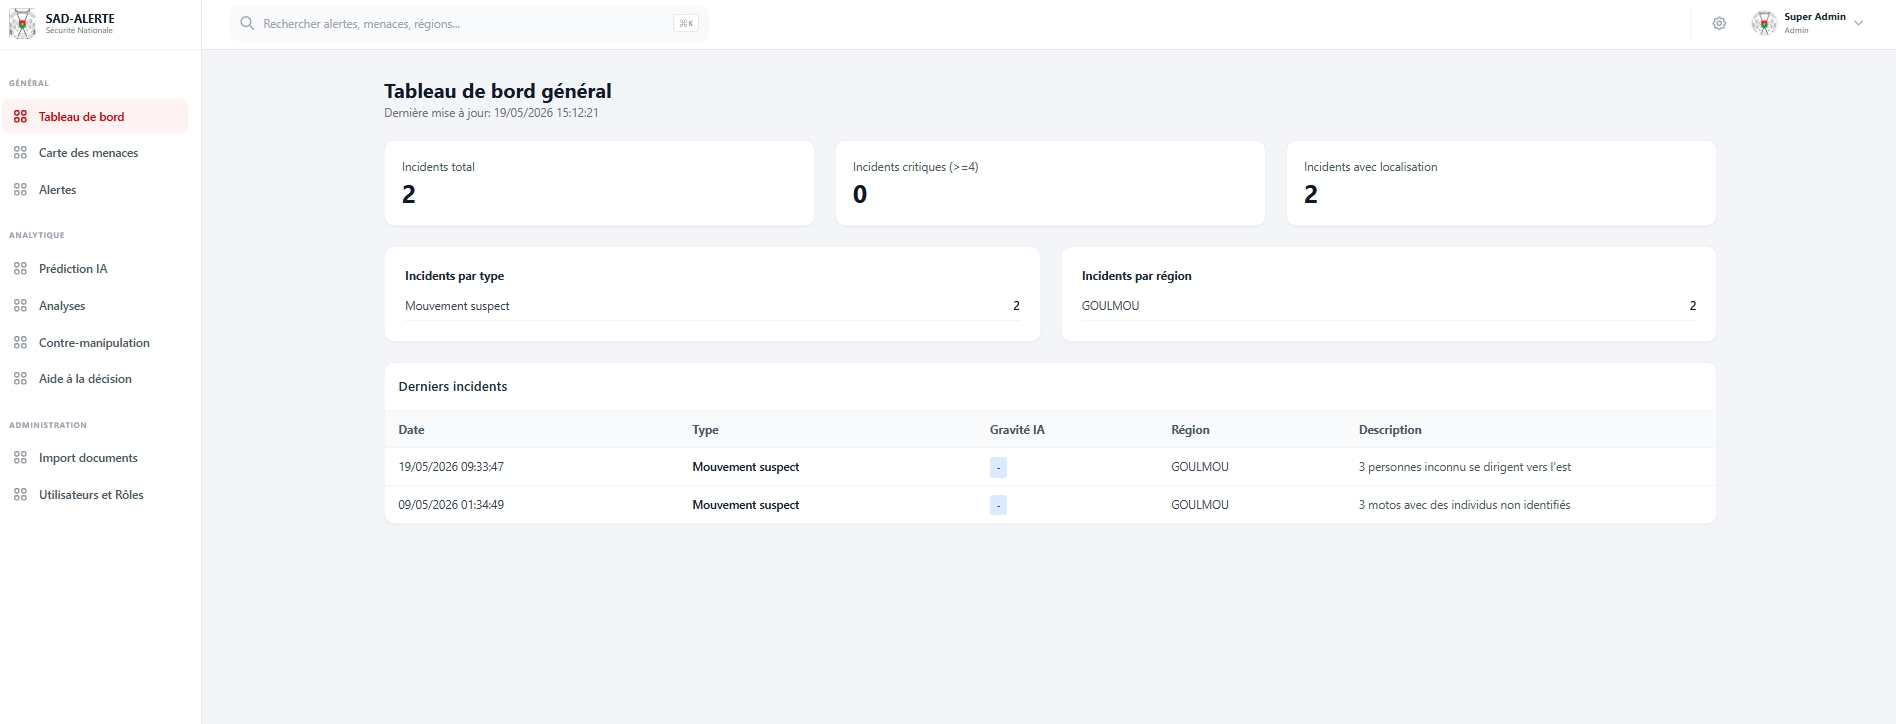
\includegraphics[width=0.9\textwidth]{media/web_dashboard_carte.png}
   \caption{Interface Web : Tableau de bord des indicateurs et cartographie interactive des incidents}
\end{figure}

\subsection{Module d'analyse et prédictions IA}
Cette section de l'application web est dédiée à l'intelligence artificielle. L'interface affiche les résultats des algorithmes de Machine Learning, notamment l'évolution des niveaux de menace et le calcul des seuils dynamiques basé sur la règle des 3 sigmas. Un tableau détaillé met en évidence les données identifiées comme aberrantes ou suspectes, permettant à l'analyste de détecter d'éventuelles tentatives de manipulation de l'information (fausses alertes).
\begin{figure}[H]
   \centering
   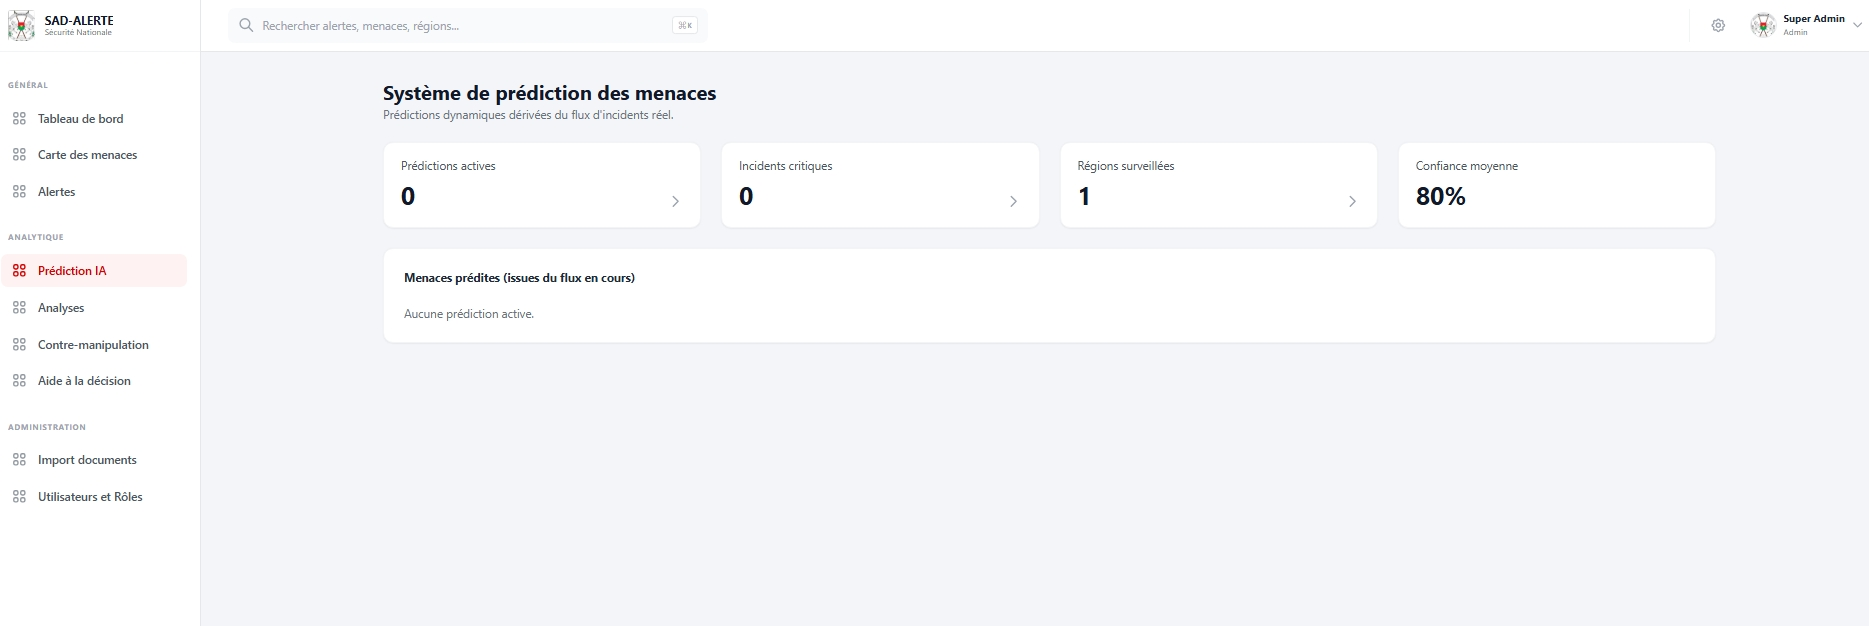
\includegraphics[width=0.9\textwidth]{media/web_ia_prediction.png}
   \caption{Interface d'analyse IA : Évaluation des seuils dynamiques et détection d'anomalies}
\end{figure}

\subsection{Import de documents et extractions}
Ce module permet la numérisation et l'exploitation des rapports administratifs textuels. L'interface propose une zone de téléversement où l'utilisateur peut importer des documents numérisés. Le système lance alors un processus d'extraction automatique pour identifier les dates, les lieux et la nature des incidents décrits. Un panneau de validation permet à l'analyste de confirmer ou de corriger les informations extraites avant leur intégration définitive dans la base de données.
\begin{figure}[H]
   \centering
   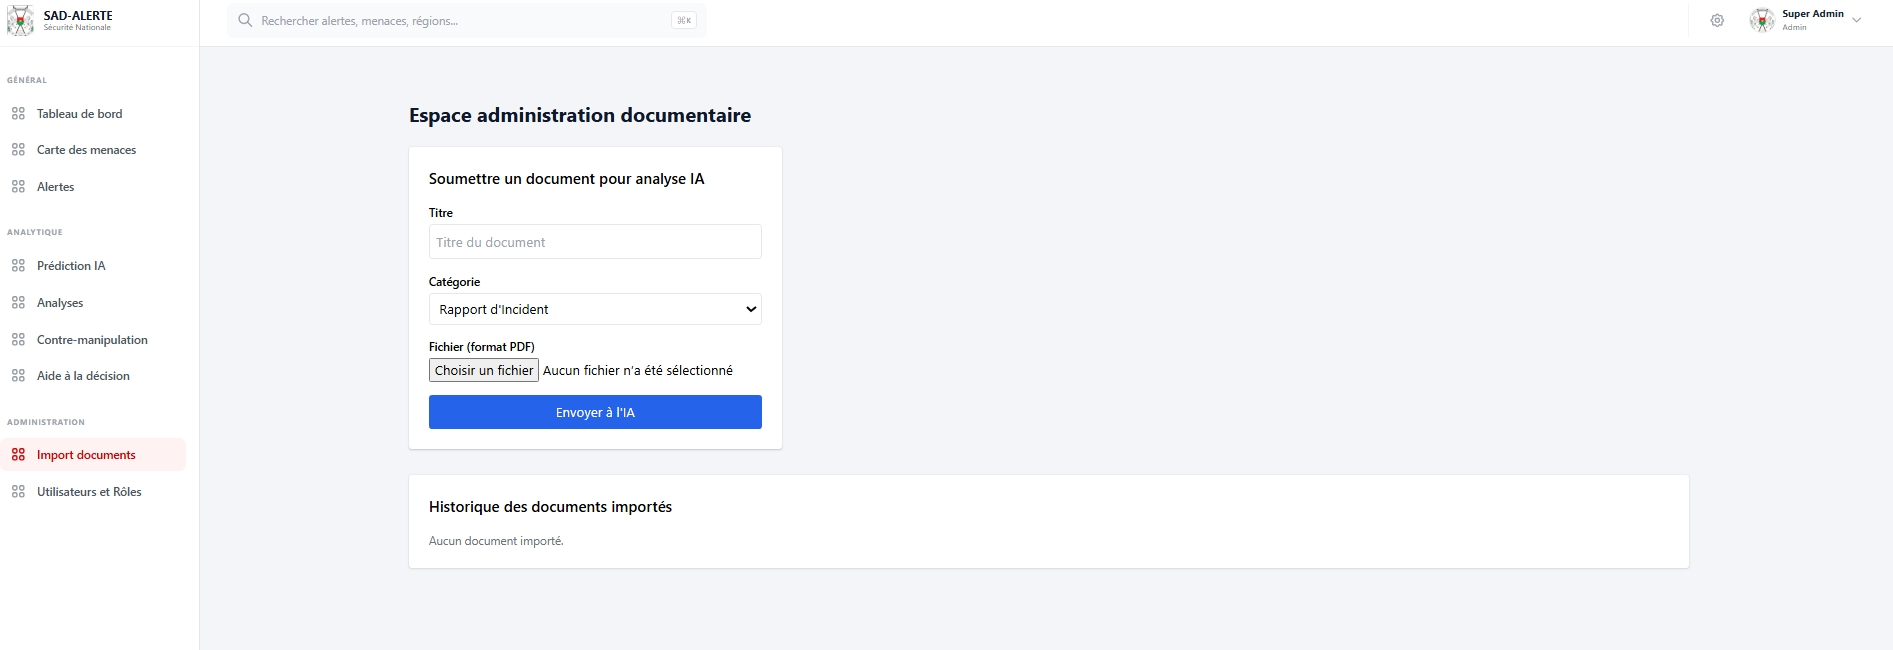
\includegraphics[width=0.9\textwidth]{media/web_import_validation.png}
   \caption{Module d'import : Téléversement de documents et validation des extractions textuelles}
\end{figure}

\subsection{Gestion des alertes et aide à la décision}
Lorsqu'un regroupement d'incidents dépasse le seuil dynamique calculé par l'IA, le système génère une alerte formelle. Cette interface de gestion centralise toutes les alertes critiques. En sélectionnant une alerte spécifique, le décideur accède à une fiche détaillée comprenant l'historique des événements liés, le niveau de fiabilité des sources et les recommandations générées par le système, facilitant ainsi la prise de décision stratégique.
\begin{figure}[H]
   \centering
   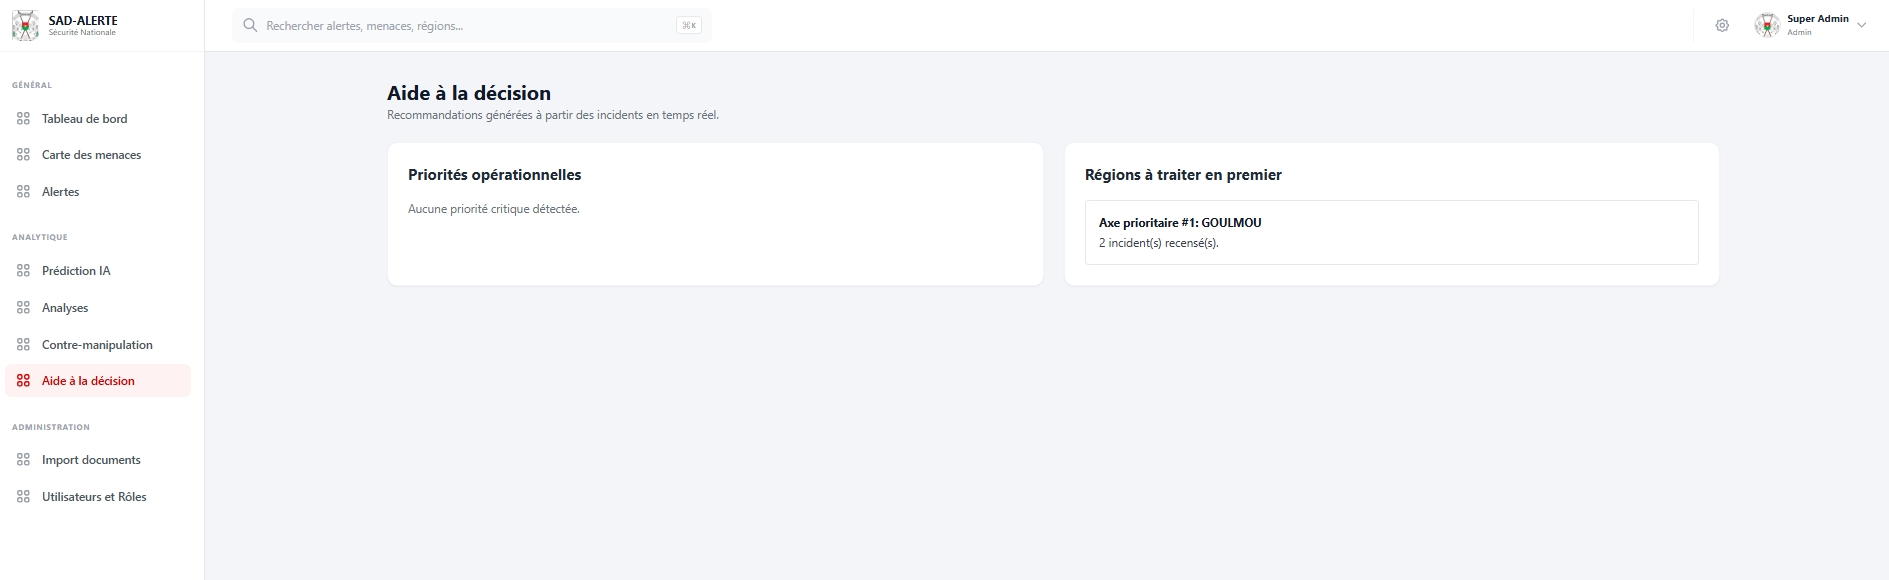
\includegraphics[width=0.9\textwidth]{media/web_alertes_decision.png}
   \caption{Interface de gestion des alertes : Aide à la décision et suivi des menaces critiques}
\end{figure}

\section{Configuration technique et matérielle}

La mise en œuvre du système SAD-ALERTE s'appuie sur des technologies modernes pour garantir performance et évolutivité :
\begin{itemize}
    \item \textbf{Application Mobile (Agent Terrain) :} Développée en \textbf{Flutter} (Dart), permettant d'avoir une application hybride fonctionnant sur Android et iOS avec une interface fluide.
    \item \textbf{Application Web (Décideurs et Administrateurs) :} Conçue avec \textbf{Next.js} et React.js, offrant un rendu rapide et une cartographie interactive pour le suivi en temps réel.
    \item \textbf{Backend (Logique serveur) :} Développé en \textbf{Node.js avec Express}, il sécurise l'accès via des tokens (JWT) et sert d'intermédiaire entre les interfaces et la base de données.
    \item \textbf{Moteur IA :} Implémenté en \textbf{Python}, il exécute les algorithmes d'apprentissage automatique, analyse les documents et identifie les fausses informations.
    \item \textbf{Base de données :} \textbf{PostgreSQL}, associé à son extension spatiale \textbf{PostGIS} pour gérer efficacement les coordonnées géographiques des signalements.
\end{itemize}

\begin{table}[H]
\centering
\caption{Configuration matérielle recommandée}
\begin{tabular}{|l|l|l|}
\hline
\textbf{Composant} & \textbf{Serveur de Production (VPS)} & \textbf{Postes utilisateurs} \\
\hline
Processeur & 4 vCPU (cœurs) minimum & Smartphone Android 8.0+ \\
\hline
RAM & 8 Go minimum & PC avec navigateur Web à jour \\
\hline
Stockage & 100 Go SSD & -- \\
\hline
Réseau & Connexion haut débit & 3G/4G pour terrain \\
\hline
\end{tabular}
\end{table}

\section{Tests et évaluation des performances}
Pour évaluer les performances du système, nous avons généré un environnement de test local. Plusieurs scénarios ont été joués :
\begin{itemize}
    \item \textbf{Tests fonctionnels :} Validation de bout en bout du flux d'authentification, de l'envoi d'alertes depuis le mobile, et de leur réception instantanée sur l'application Web.
    \item \textbf{Tests de l'Intelligence Artificielle :} Injection massive de signalements simulés pour forcer le système à adapter dynamiquement ses seuils. L'algorithme basé sur le facteur de 3 sigmas a réussi à rejeter avec succès les faux signalements en les plaçant en quarantaine, démontrant la robustesse du filtrage.
\end{itemize}

\section{Évaluation financière estimative (Budget)}
La mise en œuvre concrète de cette solution nécessite un investissement initial qui peut être estimé comme suit :

\begin{table}[H]
\centering
\caption{Estimation des coûts de déploiement annuel}
\begin{tabular}{|l|l|}
\hline
\textbf{Élément} & \textbf{Coût (FCFA)} \\
\hline
Hébergement (Serveur VPS) et nom de domaine & 250 000 \\
\hline
Services Tiers (API Cartographie, Mails SendGrid) & 50 000 \\
\hline
Conception, développement et maintenance du système & 2 000 000 \\
\hline
\textbf{Total estimatif} & \textbf{2 300 000} \\
\hline
\end{tabular}
\end{table}

Ce système représente un coût maitrisé par rapport à l'avantage stratégique et humain qu'offre l'anticipation des crises sécuritaires.

\section{Stratégie d’innovation et de déploiement}
L'intégration de ce système au sein de l'architecture sécuritaire du pays s'inscrit dans une démarche d'innovation progressive. Pour garantir son adoption, nous recommandons la stratégie de déploiement suivante :

\begin{enumerate}
    \item \textbf{Déploiement d'un prototype à périmètre réduit :} La première étape consiste à déployer une version bêta de l'application dans une seule région pilote, afin d'évaluer le comportement du système dans des conditions réelles contrôlées.
    \item \textbf{Tests de terrain avec les comités de vigilance :} Les agents locaux et les Volontaires pour la Défense de la Patrie (VDP) seront équipés de l'application mobile pour éprouver sa résilience face aux pannes de réseau et son ergonomie.
    \item \textbf{Collaboration institutionnelle avec les forces de sécurité :} Le succès du projet repose sur un partenariat étroit avec l'état-major. Les retours d'expérience des analystes militaires permettront d'affiner les modèles d'Intelligence Artificielle.
    \item \textbf{Campagne de formation des utilisateurs :} Des sessions de formation pratiques devront être organisées pour accompagner les agents dans l'appropriation de l'outil et dans la compréhension de l'importance de la rigueur de saisie.
    \item \textbf{Évaluation continue et maintenance itérative :} Enfin, un comité technique devra être mis en place pour assurer une surveillance permanente des performances des algorithmes de détection et procéder aux mises à jour nécessaires face à l'évolution des menaces.
\end{enumerate}

% CONCLUSION
\newpage
\chapter*{CONCLUSION ET PERSPECTIVES}
\addcontentsline{toc}{chapter}{CONCLUSION ET PERSPECTIVES}

Ce travail a abouti à la conception d’un système d’alerte précoce intégrant l’exploitation des données historiques, la localisation hybride, l’apprentissage automatique, la gestion dynamique des seuils et la détection des fausses informations.

Les limites incluent l’absence de déploiement réel. Les perspectives sont le développement d’un prototype opérationnel, les tests terrain, et l’extension à d’autres types d’alertes.

% RÉFÉRENCES
\newpage
\begin{thebibliography}{99}
\addcontentsline{toc}{chapter}{RÉFÉRENCES BIBLIOGRAPHIQUES}
\bibitem{geron2022} Géron A. (2022), \emph{Hands-On Machine Learning}, O'Reilly.
\bibitem{laudon2020} Laudon K. et Laudon J. (2020), \emph{Management Information Systems}, Pearson.
\bibitem{longley2015} Longley P. et al. (2015), \emph{Geographic Information Systems}, Wiley.
\bibitem{ministere2023} Ministère de la Sécurité (2023), \emph{Rapports annuels}, Ouagadougou.
\bibitem{nationsunies2006} Nations Unies (2006), \emph{Guide des systèmes d'alerte précoce}, UNISDR.
\bibitem{turban2015} Turban E. et al. (2015), \emph{Decision Support Systems}, Pearson.
\bibitem{ua2017} Union Africaine (2017), \emph{Cadre continental pour l'alerte précoce}, UA.
\bibitem{zongo2020} Zongo M. (2020), \emph{Crise sécuritaire au Burkina Faso}, Harmattan.
\end{thebibliography}

% ANNEXES
\newpage
\appendix
\chapter*{ANNEXES}
\addcontentsline{toc}{chapter}{ANNEXES}
\section*{Annexe A : Glossaire}
\section*{Annexe B : Paramètres des seuils}
\section*{Annexe C : Structure des fichiers du projet}

\end{document}